
% ----------------------------------------------------------------------
% Set the document class
% ----------------------------------------------------------------------
\documentclass[12pt]{article}
\usepackage{multirow}
\usepackage{matlab-prettifier}



% ----------------------------------------------------------------------
% Define external packages, language, margins, fonts, new commands 
% and colors
% ----------------------------------------------------------------------
\usepackage[utf8]{inputenc} % Codification
\usepackage[english]{babel} % Writing idiom

\usepackage[export]{adjustbox} % Align images
\usepackage{amsmath} % Extra commands for math mode
\usepackage{amssymb} % Mathematical symbols
\usepackage{anysize} % Personalize margins
    \marginsize{2cm}{2cm}{2cm}{2cm} % {left}{right}{above}{below}
\usepackage{appendix} % Appendices
\usepackage{cancel} % Expression cancellation
\usepackage{caption} % Captions
    \DeclareCaptionFont{newfont}{\fontfamily{cmss}\selectfont}
    \captionsetup{labelfont={bf, newfont}}
\usepackage{cite} % Citations, like [1 - 3]
\usepackage{color} % Text coloring
\usepackage{fancyhdr} % Head note and footnote
    \pagestyle{fancy}
    \fancyhf{}
    \fancyhead[L]{\footnotesize \fontfamily{cmss}\selectfont Memory Technologies} % Left of Head note
    \fancyhead[R]{\footnotesize \fontfamily{cmss}\selectfont CE5431} % Right of Head note
    \fancyfoot[L]{\footnotesize \fontfamily{cmss}\selectfont CE Dep.} % Left of Footnote
    \fancyfoot[C]{\thepage} % Center of Footnote
    \fancyfoot[R]{\footnotesize \fontfamily{cmss}\selectfont Amirkabir University of Technology} % Right of Footnote
    \renewcommand{\footrulewidth}{0.4pt} % Footnote rule
\usepackage{float} % Utilization of [H] in figures
\usepackage{graphicx} % Figures in LaTeX
\usepackage[colorlinks = true, plainpages = true, linkcolor = blue, urlcolor = blue, citecolor = blue, anchorcolor = blue]{hyperref}
\usepackage{indentfirst} % First paragraph
\usepackage[super]{nth} % Superscripts
\usepackage{siunitx} % SI units
\usepackage{subcaption} % Subfigures
\usepackage{titlesec} % Font
    \titleformat{\section}{\fontfamily{cmss}\selectfont\Large\bfseries}{\thesection}{1em}{}
    \titleformat{\subsection}{\fontfamily{cmss}\selectfont\large\bfseries}{\thesubsection}{1em}{}
    \titleformat{\subsubsection}{\fontfamily{cmss}\selectfont\normalsize\bfseries}{\thesubsubsection}{1em}{}
    \fancyfoot[C]{\fontfamily{cmss}\selectfont\thepage}

% Random text (not needed)
\usepackage{lipsum}
\usepackage{duckuments}

% New and re-newcommands
\newcommand{\sen}{\operatorname{\sen}} % Sine function definition
\newcommand{\HRule}{\rule{\linewidth}{0.5mm}} % Specific rule definition
\renewcommand{\appendixpagename}{\LARGE \fontfamily{cmss}\selectfont Appendices}

% Colors
\definecolor{istblue}{RGB}{3, 171, 230}
\definecolor{dkgreen}{rgb}{0,0.6,0}
\definecolor{gray}{rgb}{0.5,0.5,0.5}




\definecolor{bgcolor}{rgb}{0.95,0.95,0.95}

\lstset{
	backgroundcolor=\color{bgcolor},
	basicstyle=\ttfamily,
	frame=single,
	breaklines=true,
	postbreak=\mbox{\textcolor{red}{$\hookrightarrow$}\space},
}




\definecolor{codegray}{gray}{0.9}
\definecolor{codeblue}{rgb}{0.0,0.0,0.6}
\definecolor{codegreen}{rgb}{0.0,0.5,0.0}
\definecolor{codepurple}{rgb}{0.58,0.0,0.82}
\definecolor{backcolour}{rgb}{0.95,0.95,0.92}

\lstdefinestyle{mystyle}{
	backgroundcolor=\color{backcolour},
	commentstyle=\color{codegreen},
	keywordstyle=\color{codeblue},
	numberstyle=\tiny\color{codegray},
	stringstyle=\color{codepurple},
	basicstyle=\ttfamily\footnotesize,
	breakatwhitespace=false,         
	breaklines=true,                 
	captionpos=b,                    
	keepspaces=true,                 
	numbers=left,                    
	numbersep=5pt,                  
	showspaces=false,                
	showstringspaces=false,
	showtabs=false,                  
	tabsize=2
}

\lstset{style=mystyle}



% Image path
\graphicspath{ {./Images/} }
%%%%%%%%%%%%%%%%%%%%%%%%%%%%%%%%%%%%%%%%%%%%%%%%%%%%%%%%%%%%%%%%%%%%%%%%
%                                 Document                             %
%%%%%%%%%%%%%%%%%%%%%%%%%%%%%%%%%%%%%%%%%%%%%%%%%%%%%%%%%%%%%%%%%%%%%%%%
\begin{document}

% ----------------------------------------------------------------------
% Cover
% ----------------------------------------------------------------------
\begin{center}
    \begin{figure}
        \vspace{-1.0cm}
        \centering
        
\includegraphics[scale = 0.35]{Images/AUT_logo.png} % IST logo
    \end{figure}
    \mbox{}\\[2.0cm]
    \textsc{\Huge \textbf{Memory Technologies}}\\[1.0cm]
    \textsc{\LARGE Instructor: \href{https://scholar.google.com/citations?user=PAZOYiAAAAAJ&hl=en}{\textcolor{black}{Prof. Hamed Farbeh}}}\\[2.5cm]
    \textsc{\LARGE Amirkabir University of Technology} \\%\\[1.0cm]
    \textsc{(Tehran polytechnic)}
    \HRule\\[0.4cm]
    {\large \bf {\fontfamily{cmss}\selectfont Optimizing Algorithm Performance with HBM-PIM: A Matrix Multiplication Case Study} }\\[0.2cm]
    \HRule\\[1.5cm]
\end{center}

\begin{flushleft}
    \textbf{\fontfamily{cmss}\selectfont Authors:}
\end{flushleft}

\begin{center}
    \begin{minipage}{0.5\textwidth}
        \begin{flushleft}
            Morteza Adelkhani\\
            Sara Zamani
        \end{flushleft}
    \end{minipage}%
    \begin{minipage}{0.5\textwidth}
        \begin{flushright}
            \href{mailto:Madelkhani@aut.ac.ir}{\texttt{Madelkhani@aut.ac.ir}}\\
            
            \href{sara.zamani73@aut.ac.ir}{\texttt{sara.zamani73@aut.ac.ir}}
        \end{flushright}
    \end{minipage}
\end{center}

\vspace{0.5em}

\begin{flushleft}
	\textbf{\fontfamily{cmss}\selectfont Student, project by:} 
\end{flushleft}

\begin{center}
	\begin{minipage}{0.5\textwidth}
		\begin{flushleft}
			\href{https://rezaadinepour.github.io/}{\textcolor{black}{Reza Adinepour}}
		\end{flushleft}
	\end{minipage}%
	\begin{minipage}{0.5\textwidth}
		\begin{flushright}
			\href{mailto:adinepour@aut.ac.ir}{\texttt{adinepour@aut.ac.ir}}\\
		\end{flushright}
	\end{minipage}
\end{center}



    
\begin{center}
    \bigskip \bigskip \bigskip \bigskip
    \large \bf \fontfamily{cmss}\selectfont Spring 2024
\end{center}

\thispagestyle{empty}

\setcounter{page}{0}

\newpage
\section*{Evaluation, Academic Integrity and Submition}
\textbf{\textsc{Notes} on the project:}
\subsection*{1- Evaluation}
The evaluation of this project is based on the following:

\begin{enumerate}
	\item[a)] \textbf{Algorithm Implementation (10\%)}: Correctness and efficiency of the algorithm implementation.
	\item[b)] \textbf{Simulation Setup (30\%)}: Proper configuration and usage of the PIMSimulator.
	\item[c)] \textbf{Performance Analysis (30\%)}: Depth of analysis and understanding of performance metrics.
	\item[d)] \textbf{Report Quality (20\%)}: Clarity, completeness, and professionalism of the report.
	\item[e)] \textbf{Presentation (10\%)}: Effectiveness and clarity of the presentation.
\end{enumerate}

\subsection*{2- Academic Integrity}
Each student is expected to adhere to the highest standards of academic integrity. Any form of copying or plagiarism will result in severe penalties. Ensure your work is original and properly referenced.

\subsection*{3- Submission}
The project submission guideline is as follows:

\begin{enumerate}
	\item[a)] \textbf{Progress Reports}: Submit reports via the Courses portal until the deadline. Each delay in your submission is not acceptable.
	\item[b)] \textbf{Final Report and Code}: Submit your final report and source code in a zipped folder.
	\item[c)] \textbf{Presentation}: Present your findings in class during the final project meeting.
\end{enumerate}
\newpage

% ----------------------------------------------------------------------
% Contents
% ----------------------------------------------------------------------
\tableofcontents

\newpage

% ----------------------------------------------------------------------
% Body
% ----------------------------------------------------------------------

% ------------------Section 1--------------------
\section{Project Description}

\subsection{Proposed of this project:}
Neurodegenerative diseases, including Alzheimer's In this project you are going to deal with processing in memory (PIM) structure. For surfing in real-world application of PIM, in this project you have to run an algorithm on real PIM device and report your result that you get.\\
Based on the lack of accessibility of real PIM hardware you are going to using \href{https://github.com/SAITPublic/PIMSimulator}{PIMSimulator} which is based on HBM-PIM of Samsung.


\subsection{Description of HBM-PIM:}
High Bandwidth Memory (HBM) is a type of memory that's made to transfer data quickly and use less energy. It's built by stacking memory layers on top of each other, which lets them connect directly and move data fast. At the base of these layers, there's a special piece that controls the flow of data to and from other parts of the computer. HBM is often used with powerful computer chips like GPUs because it can handle a lot of data at once, making everything run smoother and faster.

Inside HBM, there are separate paths for data called pseudo-channels, and each one has smaller sections called banks where data is stored. When the computer needs to read data, it picks a specific path and bank, then grabs the data from there. This process is similar to how other types of memory work, but HBM's design lets it do this much quicker and with less energy.

Samsung has made a version of HBM called HBM-PIM that's even better because it can do some data processing right inside the memory itself. This means the computer doesn't have to move data around as much, which makes things faster and saves energy. This new design fits in with how memory is usually made, so it's easy to start using in products.

Overall, HBM and its improved version, HBM-PIM, are big steps forward for memory technology. They're really important for programs that need to process a lot of data quickly, like artificial intelligence and scientific computing, because they make everything more efficient and faster.



\section{Project Detaile}
As it described in previous section you will use the PIMSimulator to simulate the performance of different algorithms on the HBM-PIM architecture. Each student will be assigned one algorithm to analyze. The goal is to understand how PIM technology affects the performance and efficiency of these algorithms compared to traditional memory architectures. Your task to doing this project is as follow:

\subsection{Choosing Algorithm:}
You have to choose one of the following algorithms to analyze and submit it in your section of project table assignment in courses portal.

Note: \textcolor{red}{The priority of choosing an algorithm is with the first student which choose it.}


\subsubsection{Sorting Algorithms:}
\begin{enumerate}
	\item[a)] QuickSort
	\item[b)] MergeSort
	\item[c)] HeapSort
	\item[d)] Insertion Sort
	\item[e)] Bubble Sort
\end{enumerate}

\subsubsection{Graph Algorithms:}
\begin{enumerate}
	\item[a)] Dijkstra's Algorithm
	\item[b)] Breadth-First Search (BFS)
	\item[c)] Depth-First Search (DFS)
	\item[d)] Prim's Algorithm
	\item[e)] Kruskal's Algorithm
\end{enumerate}

\subsubsection{Matrix Operations:}
\begin{enumerate}
	\item[f)] Matrix Multiplication
	\item[g)] Sparse Matrix-Vector Multiplication (SpMV)
\end{enumerate}

\section*{IV. Machine Learning and Data Processing Algorithms:}
\begin{enumerate}
	\item[h)] K-means Clustering
\end{enumerate}


\subsection{Literature Review:}
Each student will review existing research on HBM, PIM, and the specific algorithm assigned to them.


\subsection{Algorithm Implementation:}
Students will implement their assigned algorithm in a compatible programming language (e.g., C++, Python) if not already available.

\subsection{Simulation Setup:}
Students will set up the PIMSimulator to run their algorithms, configuring necessary parameters and optimizing the code to leverage PIM features.

\subsection{Performance Analysis:}
Students will run simulations to collect data on execution time, power consumption, and other relevant metrics.

\subsection{Comparison:}
Compare the performance of the algorithm on HBM-PIM with traditional memory architectures.

\subsection{Report and Presentation:}
Each student will compile their findings into a detailed report and present their results to the class.




\textcolor{blue}{The algorithm I have chosen for this project is matrix multiplication. Therefore, I first need to build the simulator, the installation steps of which I will explain below:}


\section{PIMSimulator}
\subsection{Overview}
PIMSimulator is a cycle accurate model that Single Instruction, Multiple Data (SIMD) execution units that uses the bank-level parallelism in PIM Block to boost performance that would have otherwise used multiple times of bandwidth from simultaneous access of all bank. The simulator include memory and have embedded within it a PIM block, which consist of programmable command registers, general purpose register files and execution units.

Based on \href{https://github.com/umd-memsys/DRAMSim2}{\texttt{github.com/umd-memsys/DRAMSim2}}, the simulator includes the simulator includes

\begin{itemize}
	\item PIM Block:
	\begin{itemize}
		\item Register files including CRF (for command), GRF (for vector value), SRF (for scalar value)
		\item ALU (ADD, MUL, MAC, MAD, MOVE, FILL, NOP, JUMP, EXIT)
	\end{itemize}
	
	
	\item PIM Kernel:
	\begin{itemize}
		\item 
		Generate a set of memory transactions for enabling PIM operation
	\end{itemize}
	\item HBM2 support (refer to \texttt{ini/HBM2\_samsung\_2M\_16B\_x64.ini})
\end{itemize}




\subsection{HW description}
PIM is a HBM stack that is pin compatible with HBM2 and have embedded within it a PIM block

\subsubsection{Base Architecture}

\begin{figure}[h]
	\centering
	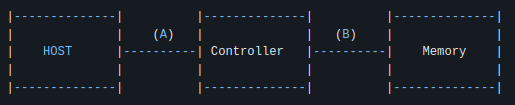
\includegraphics[width=0.8\textwidth]{Images/img2.png}
	\caption{Architecture of PIM}
	\label{fig:Architecture of PIM}
\end{figure}

\begin{itemize}
	\item Each channel is logically independent memory, so it has a dedicated independent controller.
	\item Read [Addr], Write [Addr]
	\item Activate, Read, Write, Precharge, Refresh, \texttt{Activate\_pim}, \texttt{ALU\_pim}, \texttt{Precharge\_pim}, \texttt{READ\_pim}
\end{itemize}


\begin{enumerate}
	\item HBM2
	\begin{enumerate}
		\item System Specification: \texttt{system\_hbm.ini}
		\item HBM Specification: \texttt{ini/HBM2\_samsung\_2M\_16B\_x64.ini}
		\begin{enumerate}
			\item 1 PIM block per 2 banks, 4 Bank per Bankgroup, 4 Bank group per pseudo channel, 4 pseudo channel per die, 4 die per stack.
			
			\item Prefetch size : 256bit
			
			\item burst length: 4n
			
			\item Pin speed: 2Gbps
			
			\item The simulator supports the pseudo-channel mode only, and we assume that each pseudo-channel is totally independent.
		\end{enumerate}
	\end{enumerate}
\end{enumerate}




\subsubsection{Address mapping}
\begin{enumerate}
	\item The address mapping is used when the memory controller decodes the address from host.
	\item Use Scheme8 addressing mode for PIM functionality.
	
	\texttt{|<-rank->|<-row->|<-col high->|<-bg->|<-bank->|<-chan->|<-col low->|<-offset ->|}
	
	\item the length of \texttt{col\_low} is log(BL * JEDEC\_DATA\_BUS\_BUTS/8), which are 5b both for HBM2
	
	\item You can also change the current addressing mode dynamically (Not recommended, though)
\end{enumerate}

\texttt{// Static Setting in system\_*.ini}

\texttt{ADDRESS\_MAPPING\_SCHEME=Scheme8}



\subsubsection{PIM Block Placement}
\texttt{BANKS\_PER\_PIM\_BLOCK = NUM\_BANKS / NUM\_PIM\_BLOCKS}


\begin{figure}[h]
	\centering
	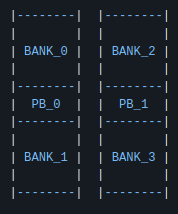
\includegraphics[width=0.3\textwidth]{Images/img3.png}
	\caption{HBM2 case}
	\label{fig:HBM2 case}
\end{figure}


\begin{enumerate}
	\item if \texttt{2 * NUM\_PIM\_BLOCKS == NUM\_BANK}, a PIM block is located per two banks.
	\begin{enumerate}
		\item \texttt{NUM\_PIM\_BLOCKS = 8, NUM\_BANKS = 16}
	\end{enumerate}
	\item if \texttt{NUM\_PIM\_BLOCKS == NUM\_BANKS}, a PIM Block (PB) is located per banks.
	\begin{enumerate}
		\item 
		\texttt{NUM\_PIM\_BLOCKS = 8, NUM\_BANKS = 8}
	\end{enumerate}
\end{enumerate}


\begin{table}[h!]
	\centering
	\begin{tabular}{|>{\centering\arraybackslash}m{1.9cm}|>{\centering\arraybackslash}m{2cm}|>{\centering\arraybackslash}m{5cm}|>{\centering\arraybackslash}m{2cm}|>{\centering\arraybackslash}m{2cm}|>{\centering\arraybackslash}m{2cm}|}
		\hline
		\textbf{Type} & \textbf{Command} & \textbf{Description} & \textbf{Result (DST)} & \textbf{Operand (SRC0)} & \textbf{Operand (SRC1)} \\ 
		\hline
		Arithmetic & ADD & addition & GRF & GRF, BANK, SRF & GRF, BANK, SRF \\ 
		\hline
		Arithmetic & MUL & multiplication & GRF & GRF, BANK, SRF & GRF, BANK, SRF \\ 
		\hline
		Arithmetic & MAC & multiply-accumulate & GRF\_B & GRF, BANK & GRF, BANK, SRF \\ 
		\hline
		Arithmetic & MAD & multiply-and-add & GRF & GRF, BANK & GRF, BANK, SRF \\ 
		\hline
		Data & MOV & load or store data from register to bank & GRF, SRF & GRF, SRF & \\ 
		\hline
		Data & FILL & copy data from bank to register & GRF, BANK & GRF, BANK & \\ 
		\hline
		Control & NOP & do nothing & & & \\ 
		\hline
		Control & JUMP & jump instruction & & & \\ 
		\hline
		Control & EXIT & exit instruction & & & \\ 
		\hline
	\end{tabular}
	\caption{Table of Commands}
	\label{tab:commands}
\end{table}


\begin{itemize}
	\item Supports RISC-style 32-bit instructions
	\item Three instructions types
	\begin{itemize}
		\item 4 Arithmetic: ADD, MUL, MAC, MAD
		\item 2 Data transfer: MOV, FILL
		\item 3 control flows: NOP, JUMP, EXIT
	\end{itemize}
	\item JUMP instruction
	\begin{itemize}
		\item Zero-cycle static branch: supports only a pre-programmed numbers of iterations
	\end{itemize}
	\item Operand type:
	\begin{itemize}
		\item Vector Register (GRF\_A, GRF\_B)
		\item Scalar Register (SRF)
		\item Bank Row Buffer
	\end{itemize}
	\item PIM instructions are stored in the Command Register File (CRF), and memory command triggers a CRF to perform a target instruction
	\begin{itemize}
		\item each memory command increments the CRF PC
	\end{itemize}
	\item DRAM commands decide where to retrieve data from DRAM for PIM arithmetic operations
\end{itemize}









\subsubsection{Movement of Data}
\begin{table}[h!]
	\centering
	\begin{tabular}{|>{\centering\arraybackslash}m{1.5cm}|>{\centering\arraybackslash}m{2.5cm}|>{\centering\arraybackslash}m{3cm}|>{\centering\arraybackslash}m{6cm}|}
		\hline
		\textbf{Mode} & \textbf{Transaction} & \textbf{PIM Instruction} & \textbf{Operation} \\ 
		\hline
		SB & Read & - & Normal Memory Read \\ 
		\hline
		SB & Write & - & Normal Memory Write \\ 
		\hline
		HAB & Write & - & PIM Write (Host to PIM Register) \\ 
		\hline
		PIM & - & MOV & read or write from bank to PIM Register \\ 
		\hline
		PIM & - & FILL & write from bank to PIM Registers \\ 
		\hline
	\end{tabular}
	\caption{Table of Transactions and Operations}
	\label{tab:transactions}
\end{table}


\begin{enumerate}
	\item SB mode: standard DRAM operation
	\item HAB mode: Allowing concurrent accesses to multiple banks with a single DRAM command
	\item PIM mode: Triggers the execution of PIM commands on the CRF by DRAM Command
\end{enumerate}





\subsection{Setup}
\subsection{Prerequisites}
\begin{itemize}
\item \texttt{Scons} tool for compiling PIMSimulator:
\begin{lstlisting}[language=bash]
	$ sudo apt install scons
\end{lstlisting}

\item \texttt{gtest} for running test cases:
\begin{lstlisting}[language=bash]
	$ sudo apt install libgtest-dev
\end{lstlisting}
\end{itemize}



\subsection{Installing}
\begin{itemize}
\item To Install PIMSimulator:
\begin{lstlisting}[language=bash]
	# compile
	scons
\end{lstlisting}
\end{itemize}



After entering the \texttt{scons} command, we encountered the following errors.
\begin{figure}[h]
	\centering
	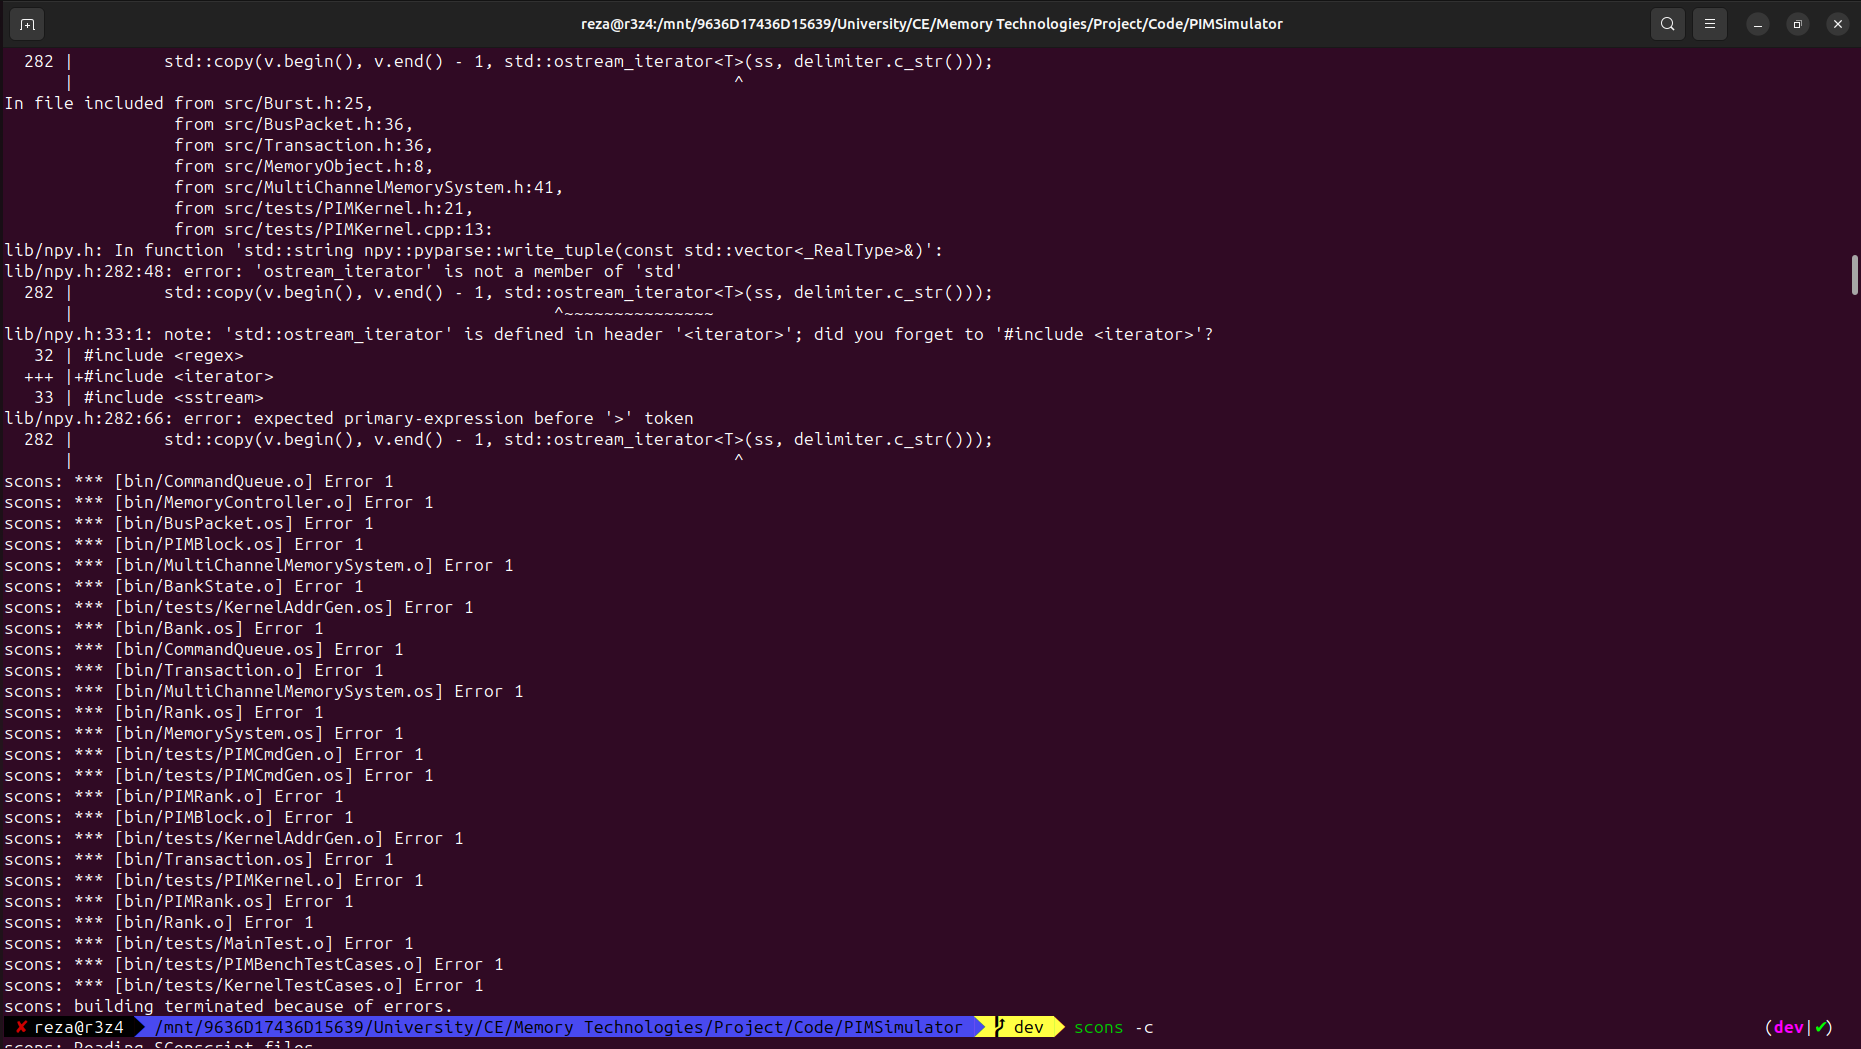
\includegraphics[width=1\textwidth]{Images/img4.png}
	\caption{Error in build}
	\label{fig:Error in build}
\end{figure}

After some investigation, I realized that the problem was with the compiler.
I had both \texttt{gcc} and \texttt{g++} compilers installed on my system, and by default, the \texttt{gcc} compiler was selected.
I changed the default compiler to \texttt{g++} with the following command, and the error problem was resolved.

\begin{lstlisting}[language=bash]
	$ sudo update-alternatives --install /usr/bin/g++ g++ /usr/bin/g++-9 60
	$ sudo update-alternatives --config g++
\end{lstlisting}

With the compiler change, the build is completed successfully

\begin{figure}[h]
	\centering
	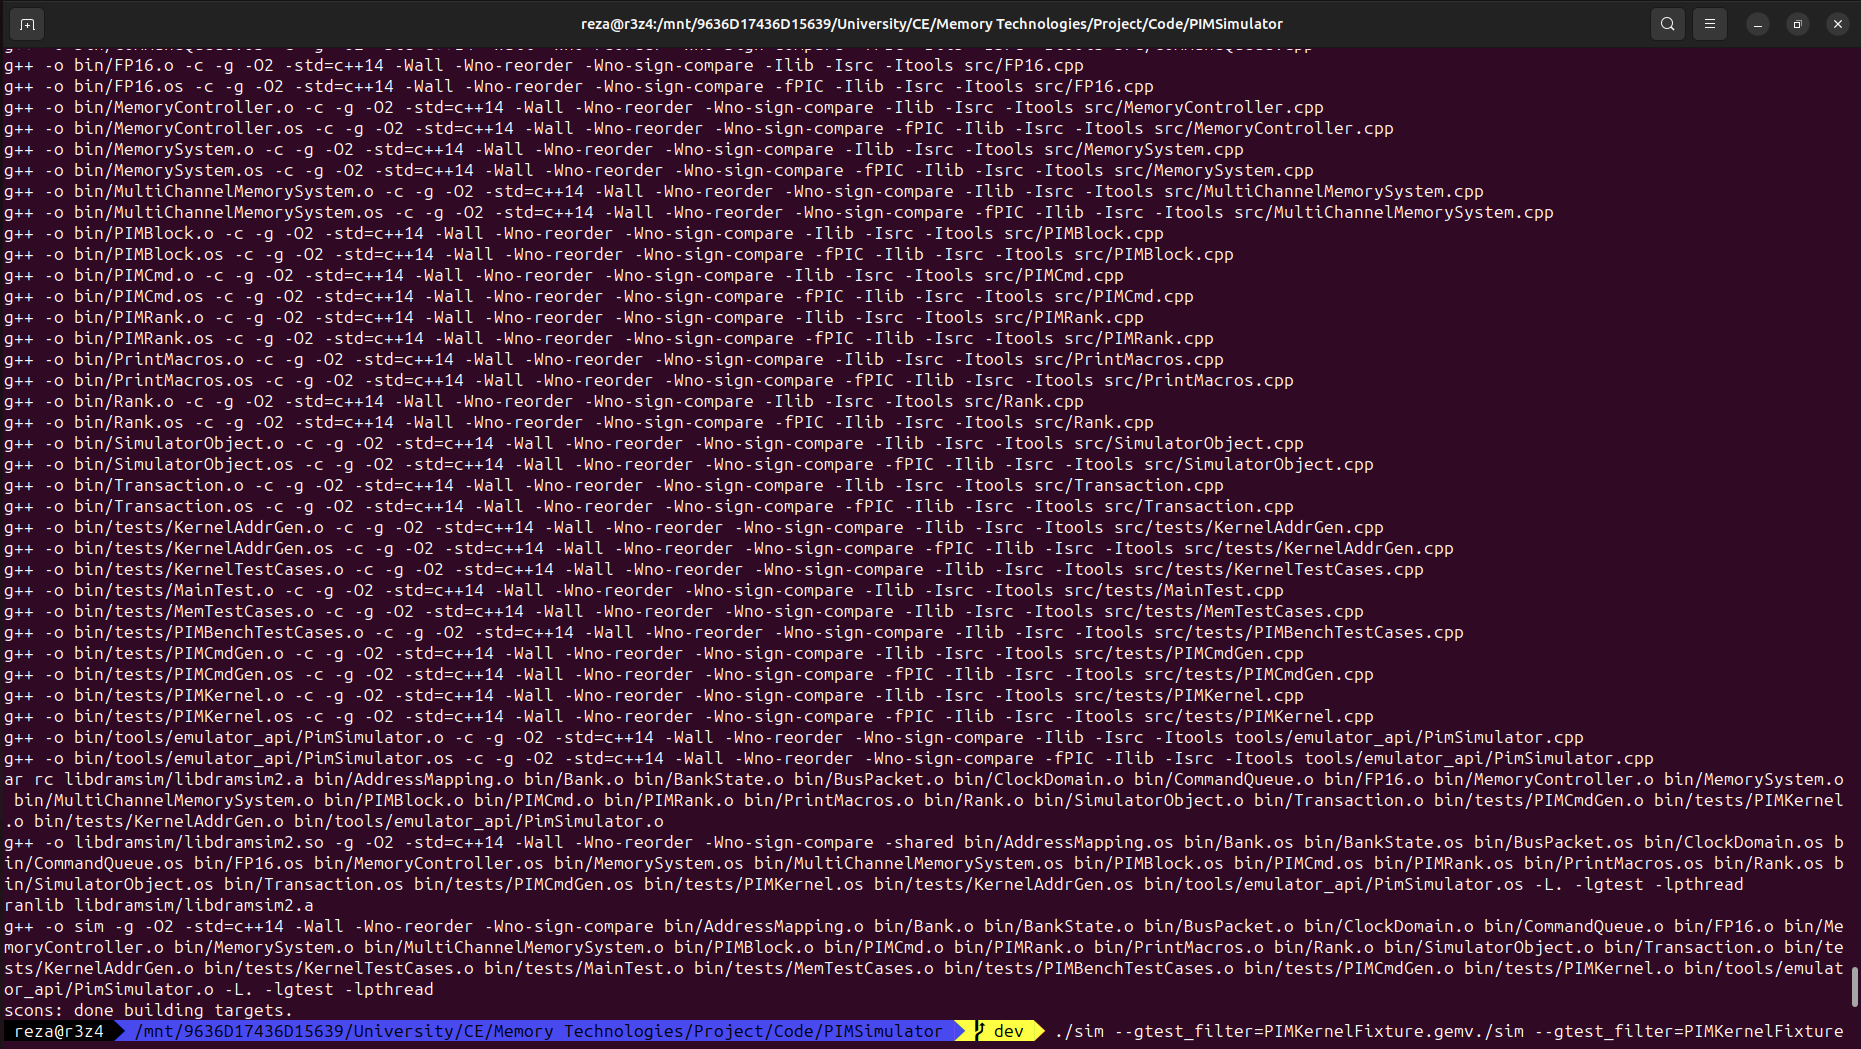
\includegraphics[width=1\textwidth]{Images/img5.png}
	\caption{Done building targets}
	\label{fig:Done building targets}
\end{figure}

In this simulator, there are pre-written examples that we can list as follows:

\subsection{Launch a Test Run}
\begin{itemize}
\item Show a list of test cases
\begin{lstlisting}[language=bash]
	./sim --gtest_list_tests
	
	# Example
	PIMKernelFixture.
	gemv_tree
	gemv
	mul
	add
	relu
	MemBandwidthFixture.
	hbm_read_bandwidth
	hbm_write_bandwidth
	PIMBenchFixture.
	gemv
	mul
	add
	relu
\end{lstlisting}
\end{itemize}



For further investigation, we will thoroughly examine and explain the matrix multiplication code file located in the path \texttt{/PIMSimulator/data/gemv/gen\_gemv.py}.




\section{Matrix-vector Multiplication Code Breakdown}

\subsection{Introduction}
This code explains a Python script that performs matrix-vector multiplication. The script involves generating random input data and weights, performing matrix multiplications, and saving the results to files.
\begin{lstlisting}[language=Python, caption=Python Code]
	import numpy as np
	
	# min dim_in = 128 -> 256bit / 16bit
	# min dim_out = 8 PIM block
	BATCH = 1
	REAL_DIM_IN = 1024
	DIM_IN = 1024
	DIM_OUT = 4096
	
	np.set_printoptions(precision=20)
	np.random.seed(41)
	
	batch_in = np.random.standard_normal(size=(DIM_IN, BATCH)).astype('float16')
	for i in range(REAL_DIM_IN, DIM_IN):
		for j in range(0, BATCH):
			batch_in[i][j] = 0
	
	data_w = np.random.standard_normal(size=(DIM_OUT, DIM_IN)).astype('float16')
	
	np.random.shuffle(data_w)
	batch_out = np.zeros((DIM_OUT, BATCH)).astype('float16')
	batch_out = np.matmul(data_w, batch_in)
	
	batch_out2 = np.zeros((DIM_OUT, BATCH)).astype('float16')
	
	for y in range(0, DIM_OUT):
		for x in range(0, DIM_IN):
			batch_out2[y] += data_w[y][x] * batch_in[x][0]
	
	batch_in = batch_in.T.copy()
	batch_out = batch_out.T.copy()
	batch_out2 = batch_out2.T.copy()
	
	np.save("gemv_input_" + str(DIM_OUT) + "x" + str(DIM_IN), batch_in)
	np.save("gemv_weight_" + str(DIM_OUT) + "x" + str(DIM_IN), data_w)
	np.save("gemv_output_" + str(DIM_OUT) + "x" + str(DIM_IN), batch_out)
	np.save("test_output_" + str(DIM_OUT) + "x" + str(DIM_IN), batch_out2)
	print(batch_in)
	print(batch_out)
	print(batch_out2)
	print(batch_in.shape)
	print(batch_out.shape)
\end{lstlisting}

\subsection{Set constants}
\begin{lstlisting}[language=Python]
	BATCH = 1
	REAL_DIM_IN = 1024
	DIM_IN = 1024
	DIM_OUT = 4096
\end{lstlisting}
\begin{itemize}
	\item \texttt{BATCH}: The batch size of the input vectors.
	\item \texttt{REAL\_DIM\_IN}: Actual input dimension size.
	\item \texttt{DIM\_IN}: Padded input dimension size (could be the same or larger than \texttt{REAL\_DIM\_IN}).
	\item \texttt{DIM\_OUT}: Output dimension size.
\end{itemize}

\subsection{Generate input data}
\begin{lstlisting}[language=Python]
	batch_in = np.random.standard_normal(size=(DIM_IN, BATCH)).astype('float16')
\end{lstlisting}
Create a \texttt{DIM\_IN x BATCH} matrix filled with random values from a standard normal distribution, converted to \texttt{float16} precision.

\subsection{Zero out the padded part of the input}
\begin{lstlisting}[language=Python]
	for i in range(REAL_DIM_IN, DIM_IN):
		for j in range(0, BATCH):
			batch_in[i][j] = 0
\end{lstlisting}
Set the elements of \texttt{batch\_in} to zero for indices from \texttt{REAL\_DIM\_IN} to \texttt{DIM\_IN} to handle the padded part.

\subsection{Generate weight data}
\begin{lstlisting}[language=Python]
	data_w = np.random.standard_normal(size=(DIM_OUT, DIM_IN)).astype('float16')
	np.random.shuffle(data_w)
\end{lstlisting}
Create a \texttt{DIM\_OUT x DIM\_IN} matrix filled with random values from a standard normal distribution, converted to \texttt{float16} precision. Shuffle the rows of \texttt{data\_w}.

\subsection{Initialize output matrices and perform matrix multiplication}
\begin{lstlisting}[language=Python]
	batch_out = np.zeros((DIM_OUT, BATCH)).astype('float16')
	batch_out = np.matmul(data_w, batch_in)
\end{lstlisting}

\subsection{Manual matrix multiplication for verification}
\begin{lstlisting}[language=Python]
	batch_out2 = np.zeros((DIM_OUT, BATCH)).astype('float16')
	
	for y in range(0, DIM_OUT):
		for x in range(0, DIM_IN):
			batch_out2[y] += data_w[y][x] * batch_in[x][0]
\end{lstlisting}
\texttt{batch\_out2} is calculated element-wise by iterating over each element of the result and summing the product of corresponding elements from \texttt{data\_w} and \texttt{batch\_in}.

\subsection{Transpose the input and output matrices}
\begin{lstlisting}[language=Python]
	batch_in = batch_in.T.copy()
	batch_out = batch_out.T.copy()
	batch_out2 = batch_out2.T.copy()
\end{lstlisting}

\subsection{Save the input, weight, and output matrices to files}
\begin{lstlisting}[language=Python]
	np.save("gemv_input_" + str(DIM_OUT) + "x" + str(DIM_IN), batch_in)
	np.save("gemv_weight_" + str(DIM_OUT) + "x" + str(DIM_IN), data_w)
	np.save("gemv_output_" + str(DIM_OUT) + "x" + str(DIM_IN), batch_out)
	np.save("test_output_" + str(DIM_OUT) + "x" + str(DIM_IN), batch_out2)
\end{lstlisting}

\subsection{Print the matrices and their shapes}
\begin{lstlisting}[language=Python]
	print(batch_in)
	print(batch_out)
	print(batch_out2)
	print(batch_in.shape)
	print(batch_out.shape)
\end{lstlisting}


After running the code, the output is as follows, and the matrices are saved as Numpy arrays in the same directory.

\begin{figure}[h]
	\centering
	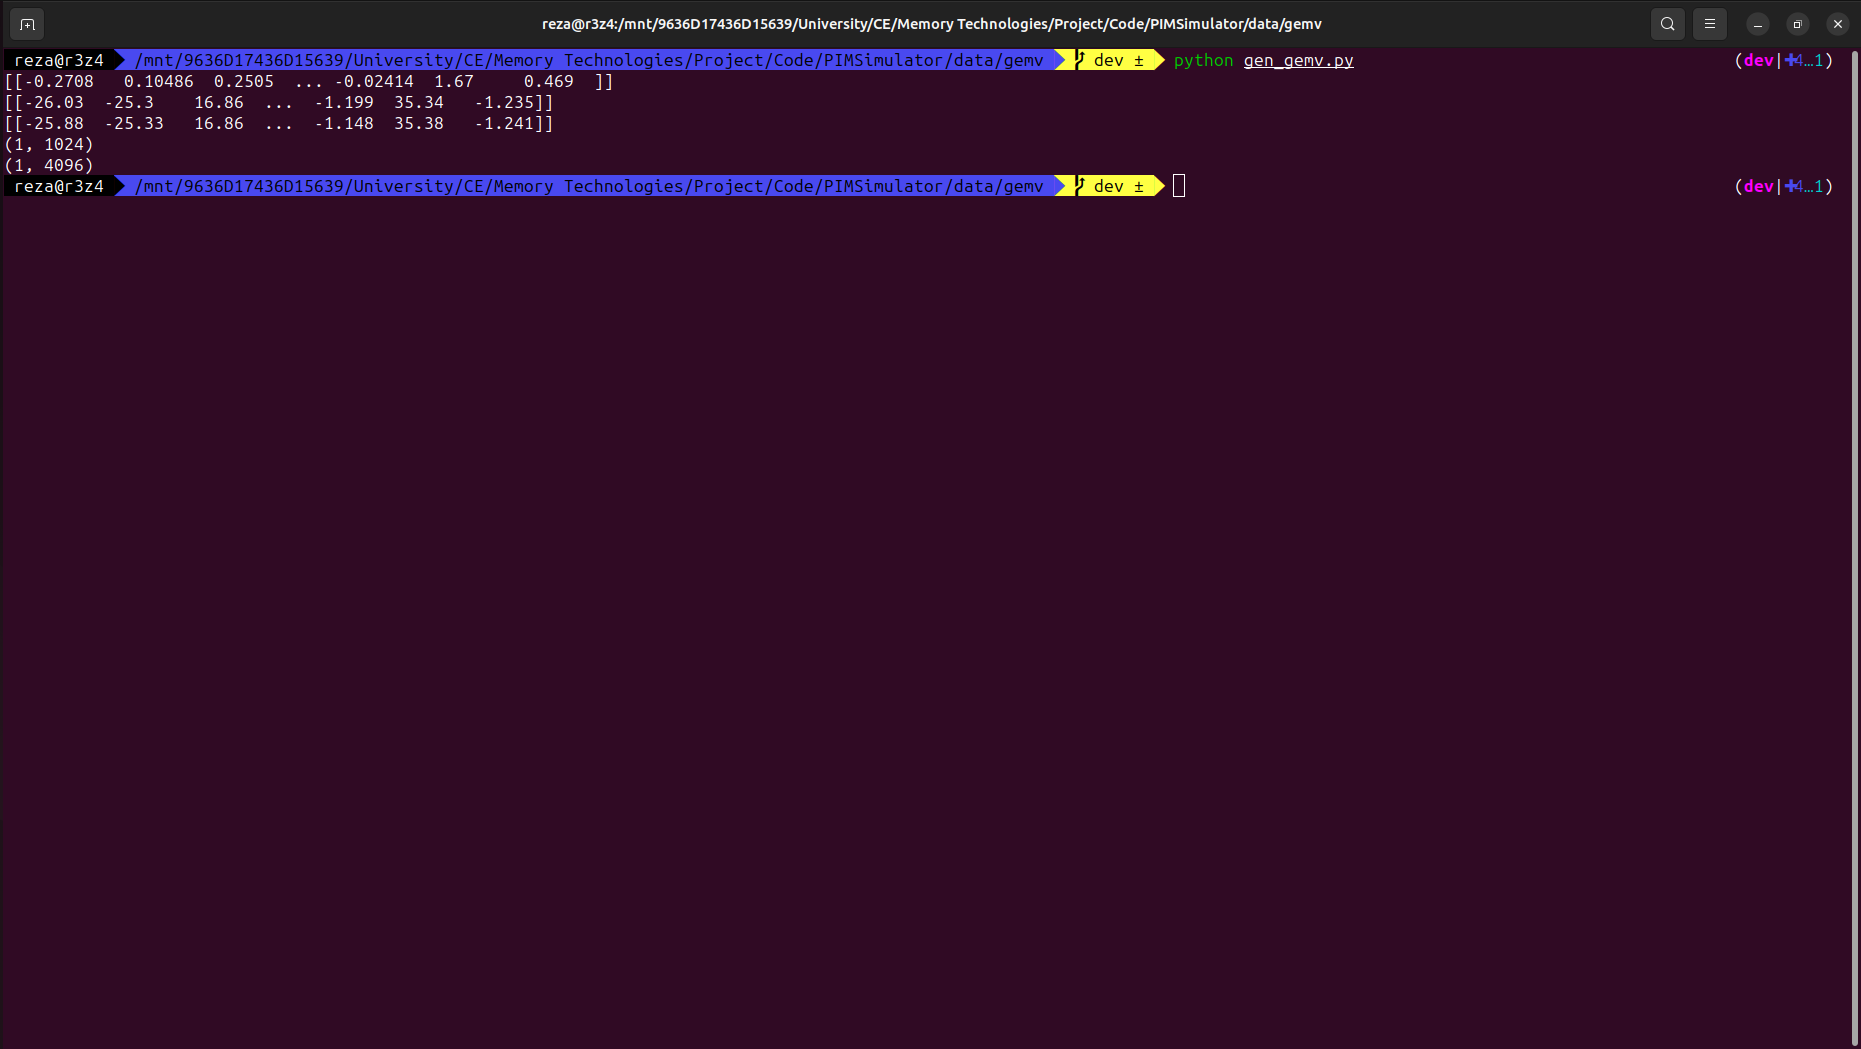
\includegraphics[width=0.8\textwidth]{Images/img6.png}
	\caption{Output of \texttt{gen\_gemv.py}}
	\label{fig:Output of gen_gemv.py}
\end{figure}


Now, after preparing the matrices, it is time to perform the matrix multiplication once with PIM and once without PIM.

To do this, we enter the following command in the simulator directory.
The simulator runs the program once without considering PIM and once with considering PIM, and displays the outputs.

\begin{lstlisting}[language=bash]
	$ ./sim --gtest_filter=PIMBenchFixture.gemv
\end{lstlisting}


\newpage










\section{Output simulation}
The simulation output is as follows:
\begin{figure}[h]
	\centering
	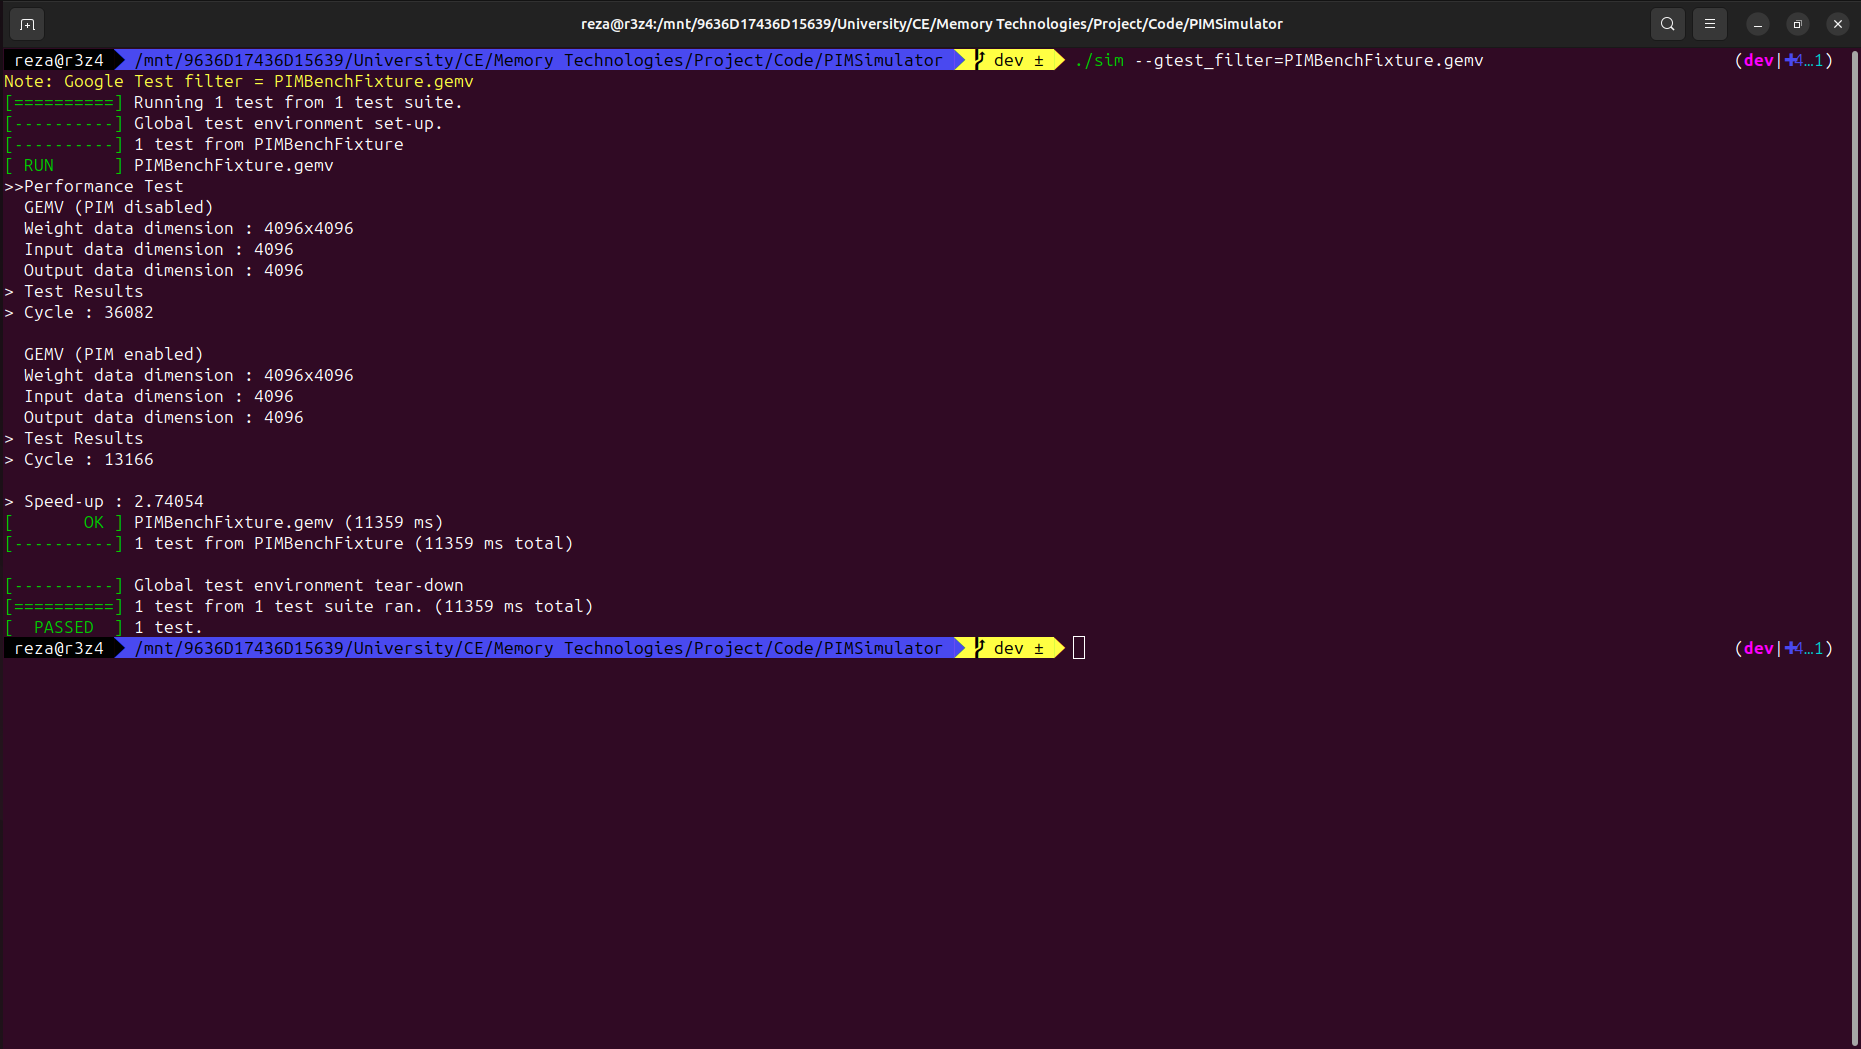
\includegraphics[width=0.8\textwidth]{Images/img7.png}
	\caption{Output of PIM simulation}
	\label{fig:Output of PIM simulation}
\end{figure}


\subsection{Analysis}

\subsubsection{Test Context}
The test involves one test suite named \texttt{PIMBenchFixture} with one test case \texttt{gemv}. The simulation was executed using Google Test with the filter \texttt{PIMBenchFixture.gemv}.

\subsubsection{Performance Test}
The GEMV operation was performed twice:
\begin{enumerate}
	\item \textbf{Without PIM:}
	\begin{itemize}
		\item \textbf{Weight Data Dimension:} 4096x4096
		\item \textbf{Input Data Dimension:} 4096
		\item \textbf{Output Data Dimension:} 4096
		\item \textbf{Cycles:} 36,082
	\end{itemize}
	\item \textbf{With PIM:}
	\begin{itemize}
		\item \textbf{Weight Data Dimension:} 4096x4096
		\item \textbf{Input Data Dimension:} 4096
		\item \textbf{Output Data Dimension:} 4096
		\item \textbf{Cycles:} 13,166
	\end{itemize}
\end{enumerate}

\subsubsection{Results Interpretation}
\begin{itemize}
	\item \textbf{Cycle Count:}
	\begin{itemize}
		\item \textbf{Without PIM:} The matrix multiplication took 36,082 cycles.
		\item \textbf{With PIM:} The matrix multiplication took 13,166 cycles.
	\end{itemize}
	\item \textbf{Speed-up:} The speed-up achieved by enabling PIM is calculated as 2.74054.
\end{itemize}

\subsubsection{Overall Test Duration}
The total time taken for the test execution was 11,359 milliseconds.


\subsubsection{Significant Performance Improvement}
The use of PIM technology resulted in a substantial reduction in the number of cycles required to complete the GEMV operation. Specifically, PIM enabled a 2.74x speed-up compared to the traditional approach without PIM. This indicates that PIM technology can significantly enhance the performance of matrix-vector multiplication by reducing the cycle count, which directly correlates to faster computation times.

\subsubsection{Consistency in Data Dimensions}
The dimensions of the weight, input, and output data were consistent across both tests (4096x4096 for weight and 4096 for both input and output). This ensures a fair comparison between the PIM-enabled and PIM-disabled scenarios.

\subsubsection{Total Execution Time}
The entire test suite, including setup and teardown, completed in approximately 11.359 seconds. This time includes not only the GEMV operations but also any additional overhead associated with the test framework and simulation environment.

\subsubsection{Pass/Fail Status}
The test passed successfully, indicating that the GEMV functionality works as expected in both PIM-enabled and PIM-disabled modes.







\section{Conclusion}
The simulation results clearly demonstrate the performance benefits of utilizing PIM technology for matrix-vector multiplication tasks. By significantly reducing the number of cycles required for the GEMV operation, PIM can lead to faster computations and more efficient processing, making it a valuable approach for high-performance computing applications.

The successful completion of this test and the observed speed-up highlight the potential of PIM technology in accelerating matrix operations, which are fundamental in various computational workloads, including machine learning and scientific computing.




%\cite{PIMSimulator}\cite{SAIT}\cite{DRAMSim2}






\newpage
% ----------------------------------------------------------------------
% References
% ----------------------------------------------------------------------
\bibliographystyle{plain}
\bibliography{refs}

\end{document}